\documentclass{beamer}
%\usepackage[margin=1.0in]{geometry}

\usepackage[utf8]{inputenc}
\usepackage[magyar]{babel}
\usepackage[T1]{fontenc}
\usepackage{lmodern}

%----------------------------------------------------------------------------------------
%	MATH PACKAGES
%----------------------------------------------------------------------------------------

% Banish \phi from this realm
\renewcommand{\phi}{\varphi}

\usepackage{amsmath, amssymb, mathrsfs}
\usepackage{mathtools}

%----------------------------------------------------------------------------------------
%	DEFINING NEW FUNCTIONS
%----------------------------------------------------------------------------------------

% --------- MATH MODE ---------
% Equation numbering per section
\numberwithin{equation}{section}

% \cdot instead of asterisk (*) symbol
\mathcode`\*="8000
{\catcode`\*\active\gdef*{\cdot}}

% --------- OTHER ---------

% Quotes
\usepackage[autostyle=false]{csquotes}
\newcommand{\q}[1]{„#1''} % Redefine quotations

\usetheme{Madrid}
\usecolortheme{default}
\setbeamertemplate{caption}[numbered]

\newif\ifplacelogo
\placelogotrue
%----------------------------------------------------------------------------------------
%	TITLE PAGE
%----------------------------------------------------------------------------------------
\title[Cosmic Microwave Background]
{Power spectrum of the\\Cosmic Microwave Background radiation}

%\subtitle{Data Science Laboratory}

\author[Balázs Pál]
{Balázs Pál\inst{1}}

\institute[ELTE]
{
  \inst{1}
  Eötvös Loránd University
}

\date[ELTE 2020]
{Data Science Laboratory, October 2020}

%\logo{\includegraphics[height=1.5cm]{lion-logo.jpg}}

\begin{document}

\frame{\titlepage}
%----------------------------------------------------------------------------------------
%	SLIDE 1.
%----------------------------------------------------------------------------------------
\begin{frame}

\begin{figure}
	\includegraphics[width=1.0\textwidth]{images/cmb_ang_spec_map_orig.png}
\end{figure}

\end{frame}
%----------------------------------------------------------------------------------------
%	SLIDE 2.
%----------------------------------------------------------------------------------------
\begin{frame}
\frametitle{Theoretical considerations}

\begin{itemize}
	\item Black-body radiation  with average colour temperature of $2.725 \mathrm{K}$
	\item Study is somewhat analogous to the H atom
\end{itemize}

\end{frame}
\placelogofalse
%----------------------------------------------------------------------------------------
%	SLIDE 3.
%----------------------------------------------------------------------------------------
\begin{frame}
\frametitle{Theoretical considerations}

\begin{figure}
	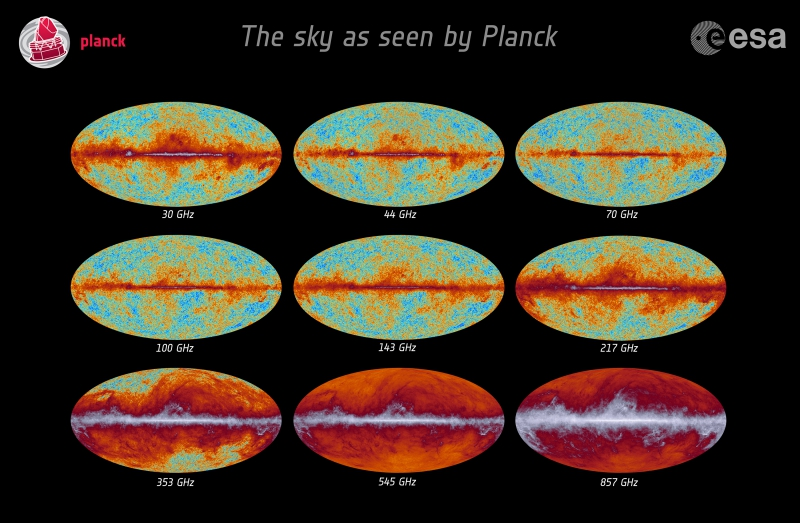
\includegraphics[width=1.0\textwidth]{images/planck_frequency_channels.jpg}
\end{figure}

\end{frame}
%----------------------------------------------------------------------------------------
%	SLIDE 4.
%----------------------------------------------------------------------------------------
\begin{frame}
\frametitle{Datasets used}

\begin{block}{Simulation}
	\begin{itemize}
		\item Power spectrum
	\end{itemize}
\end{block}

\begin{alertblock}{Analysis of measurements}
	\begin{itemize}
		\item Planck
	\end{itemize}
\end{alertblock}

\end{frame}
%----------------------------------------------------------------------------------------
%	SLIDE 5.
%----------------------------------------------------------------------------------------
\begin{frame}
\frametitle{Sample outputs of method II. - Foreground sources}

\begin{figure}
	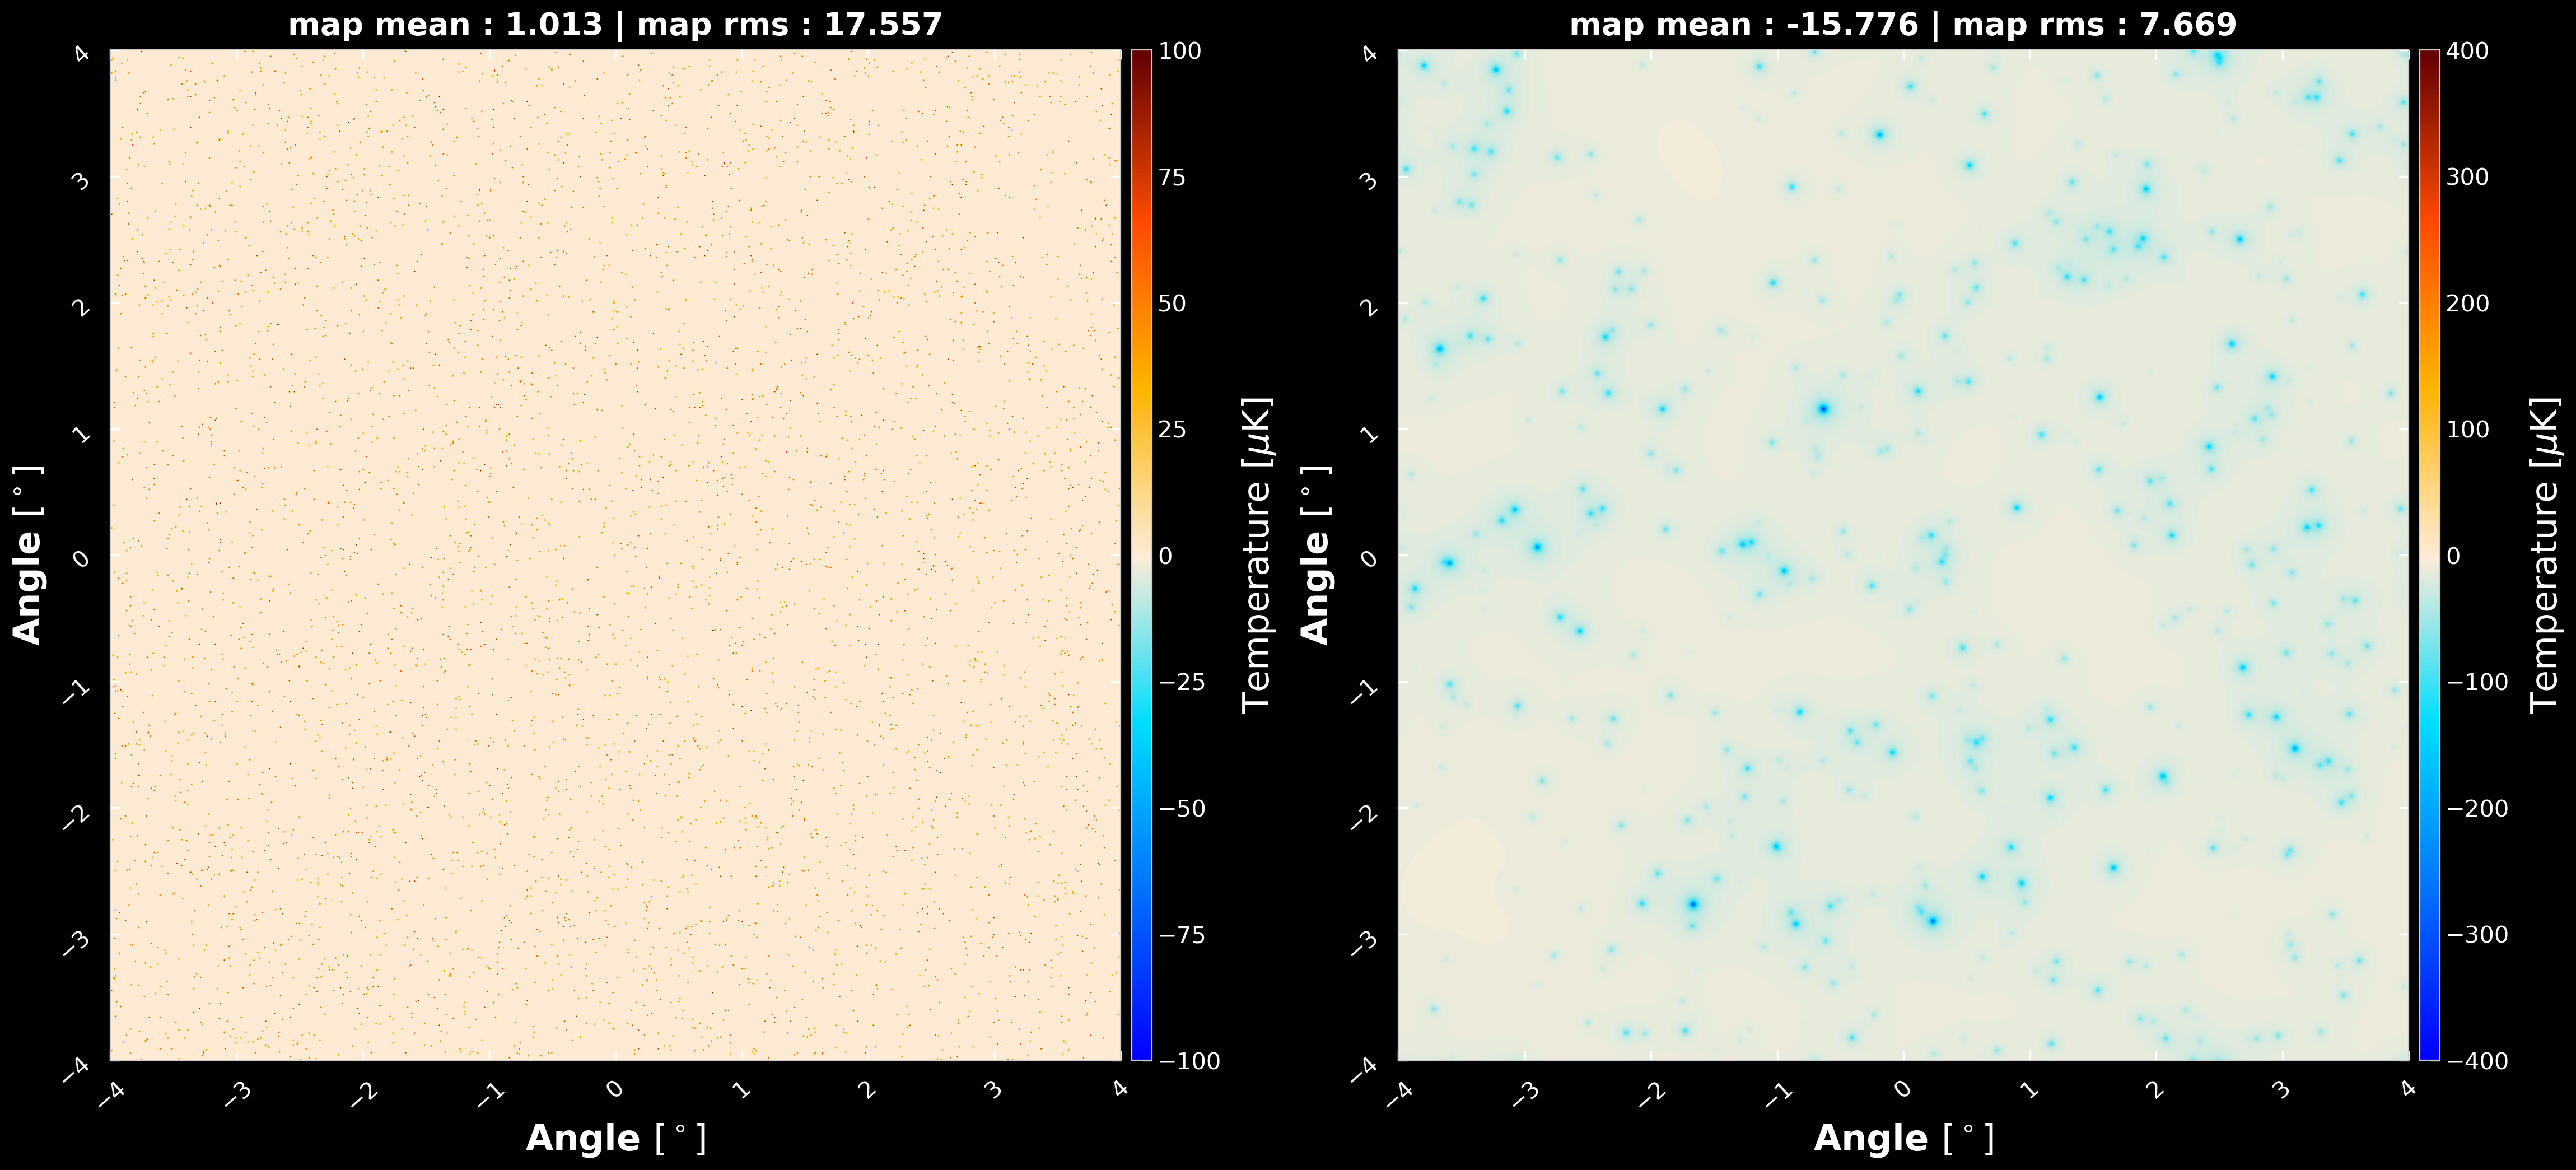
\includegraphics[width=\textwidth]{./images/CMB_sim_foregrounds_concat.png}
	\captionof{figure}{Randomly generated point sources (left) and the randomly generated map of the thermal component of the Sunyaev-Zeldovich effect (right).}
\end{figure}

\end{frame}
%----------------------------------------------------------------------------------------
%	SLIDE 6.
%----------------------------------------------------------------------------------------
\begin{frame}
\frametitle{CMB generation -- first method}

\begin{figure}[ht]
\centering
	\includegraphics[width=0.9\textwidth]{./images/CMB_I_map_gen_1.png}
	\captionof{figure}{Randomly generated full-sky intensity map of the CMB temperature anisotropy using HEALPix routines and conventions.}
\end{figure}

\end{frame}

%----------------------------------------------------------------------------------------
%	SLIDE 7.
%----------------------------------------------------------------------------------------
\begin{frame}
\frametitle{Sample outputs of method II. - Noises}

\begin{figure}
	\includegraphics[width=\textwidth]{./images/noise_compare.png}
	\captionof{figure}{The different noise components in the simulation. All noises here are considered to be Gaussian.}
\end{figure}

\end{frame}



%----------------------------------------------------------------------------------------
%	SLIDE 8.
%----------------------------------------------------------------------------------------
\begin{frame}
\frametitle{Reconstructed angular power spectrum}

\begin{figure}
	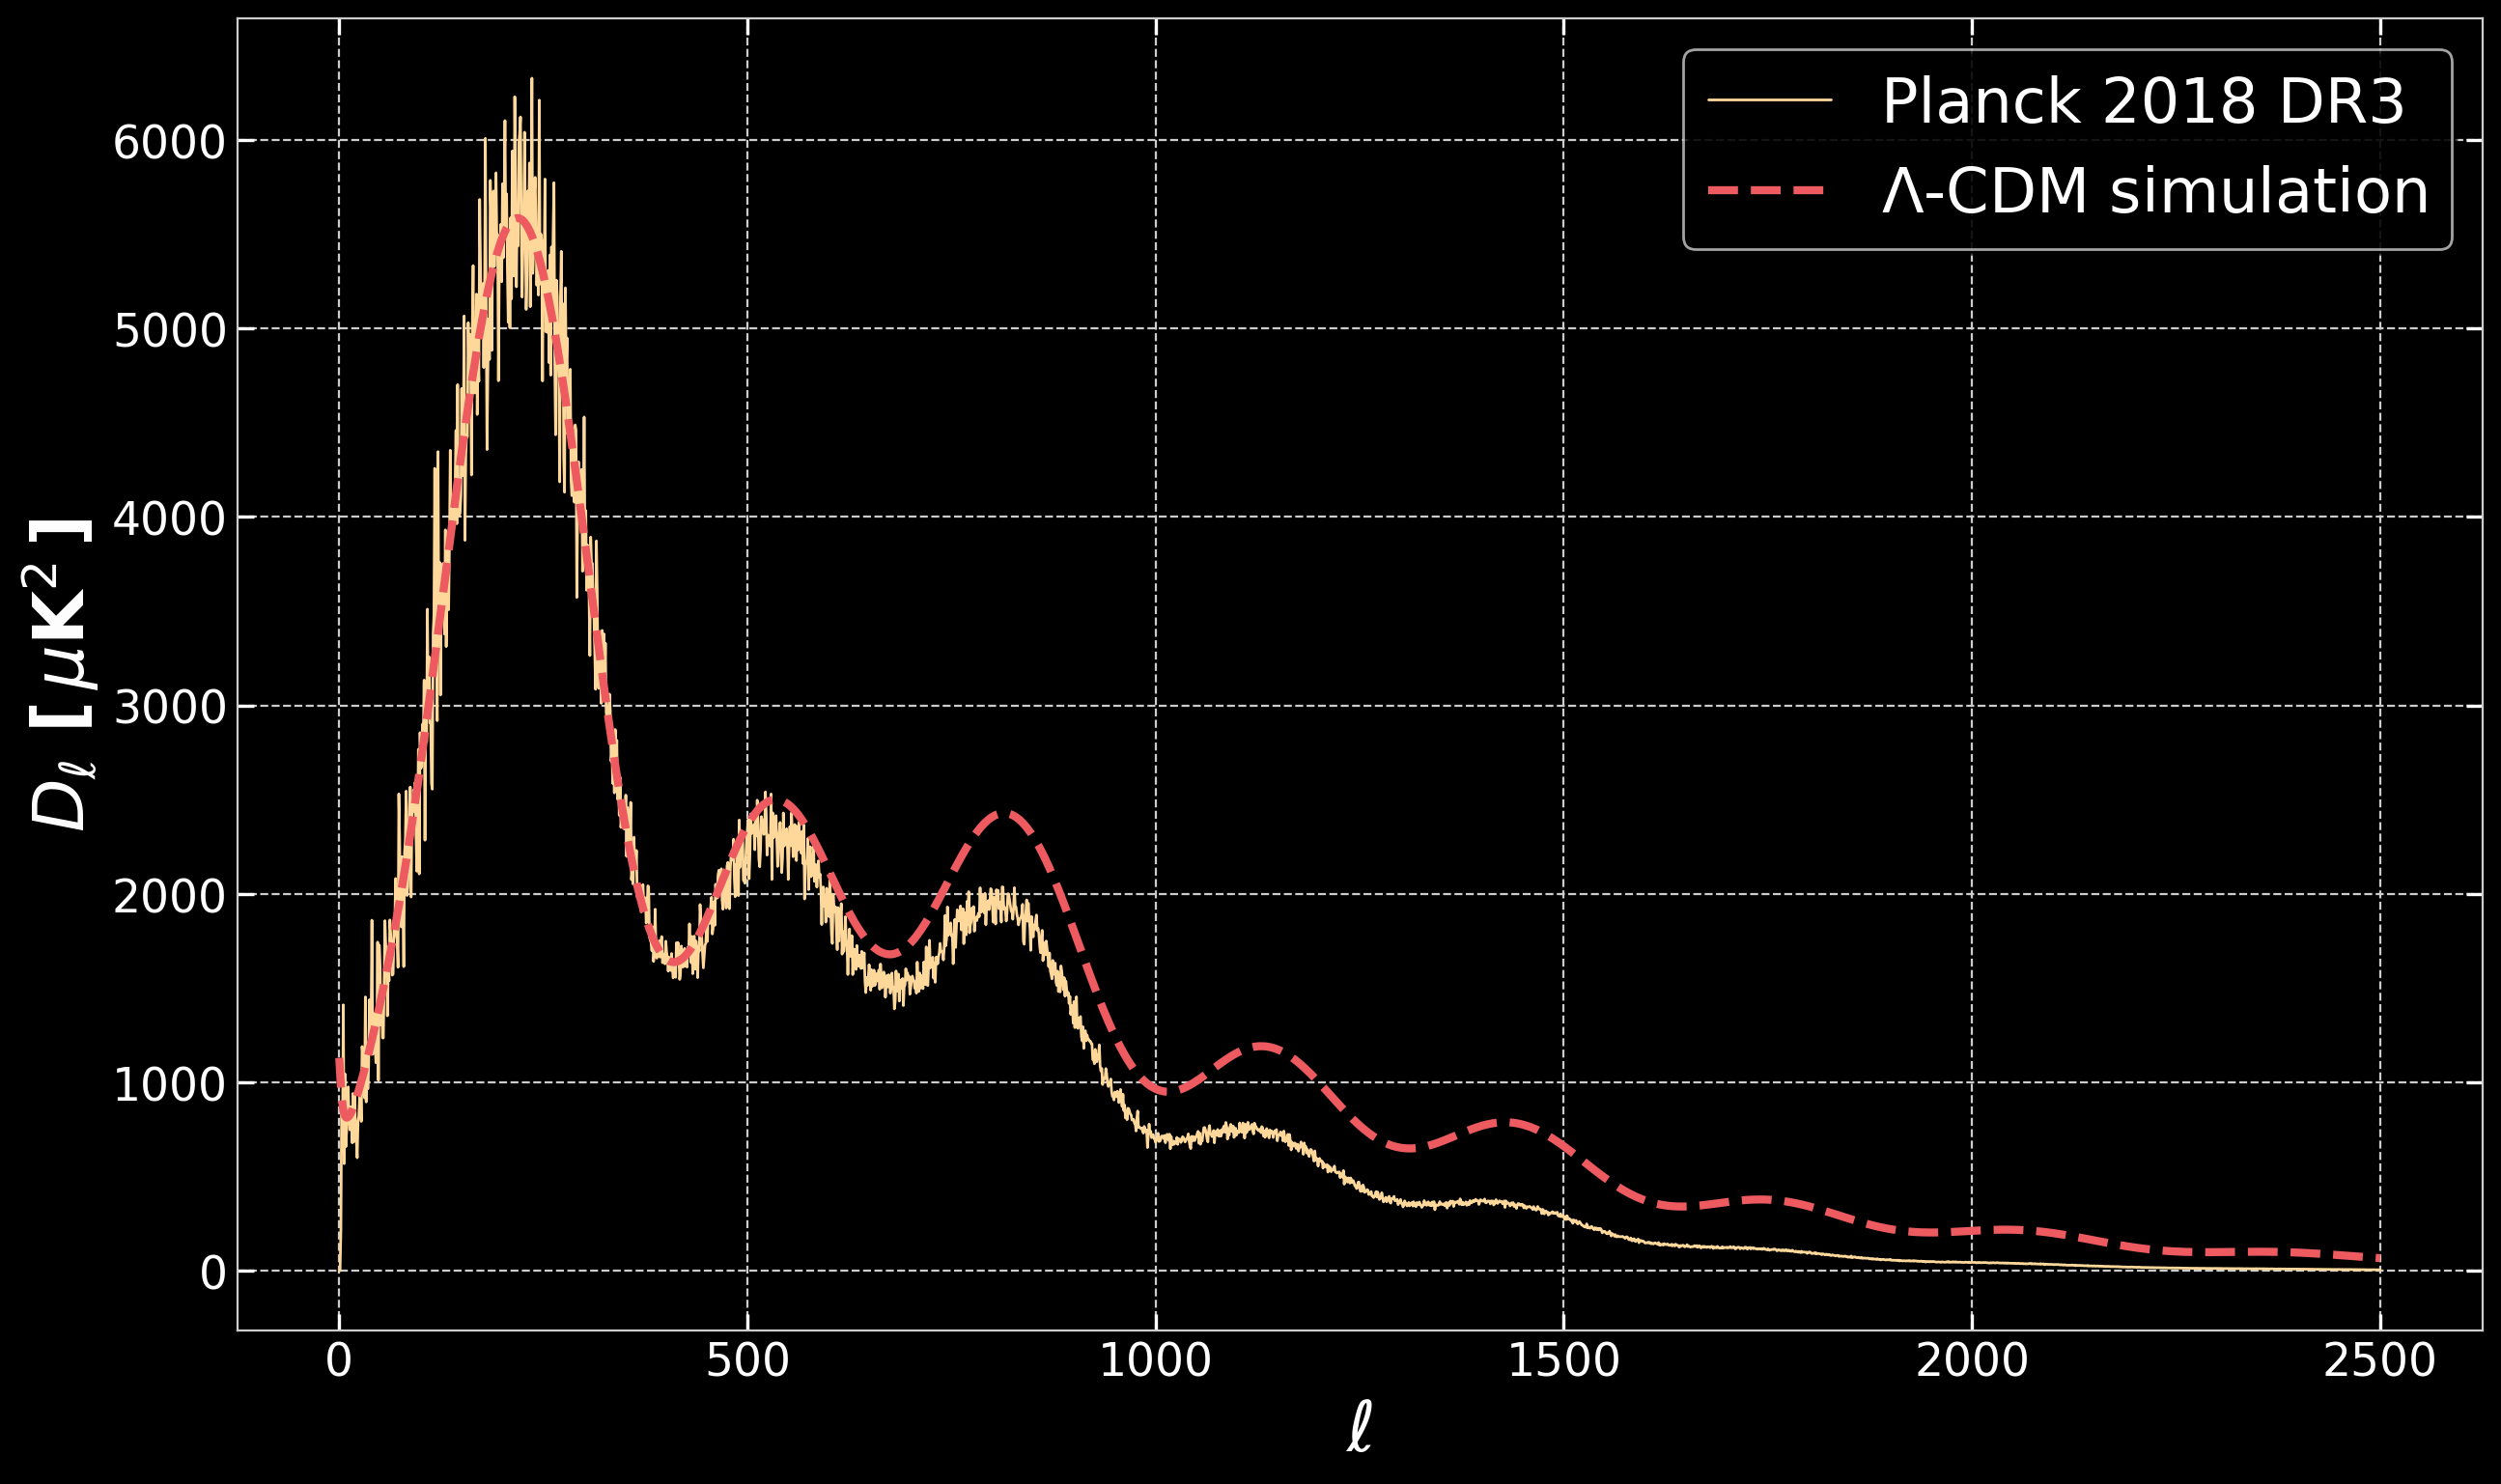
\includegraphics[width=0.9\textwidth]{images/cmb_angular_spectrum_planck_2018.png}
\end{figure}

\end{frame}


%----------------------------------------------------------------------------------------
%	SLIDE 9.
%----------------------------------------------------------------------------------------
\begin{frame}
\frametitle{MCMC algorithm tries to find cosmological parameters...}

\begin{figure}
	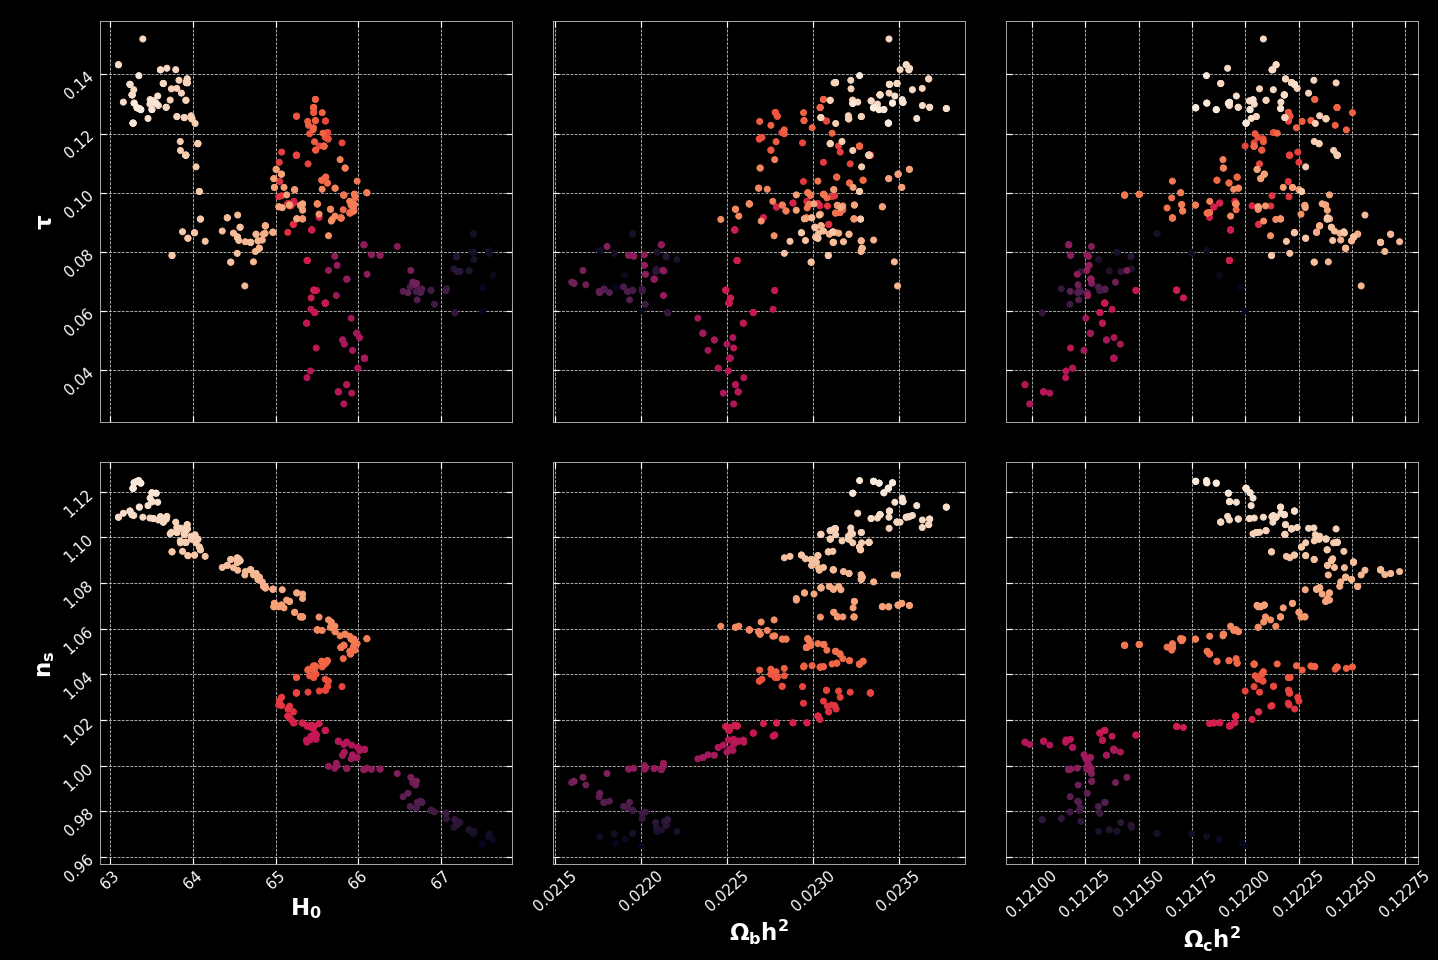
\includegraphics[width=0.9\textwidth]{images/mcmc.png}
\end{figure}

\end{frame}




\end{document}